% SpongeBatchHasher(width=B, rate=4), as in circuits/hasher_sponge.circom.
%
% Standalone: compile with pdflatex/xelatex for a cropped PDF, or drop the
% tikzpicture into a figure environment in the paper.
%
% \usepackage{tikz} \usetikzlibrary{arrows.meta,positioning,calc,fit}
\documentclass[tikz,border=4pt]{standalone}
\usepackage{tikz}
\usetikzlibrary{arrows.meta,positioning,calc,fit,backgrounds}

\begin{document}
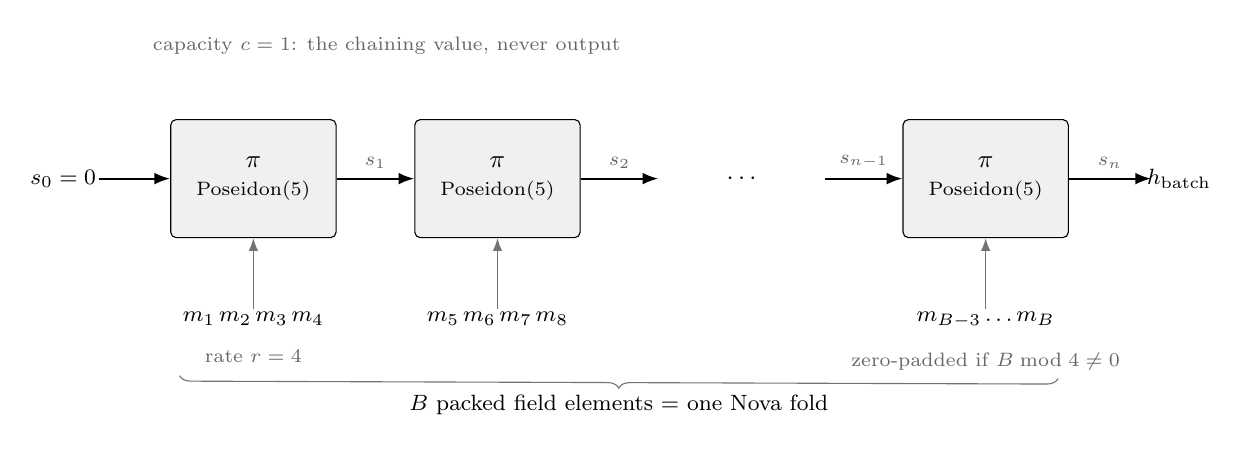
\begin{tikzpicture}[
  font=\small,
  perm/.style={
    draw, rounded corners=2pt, fill=black!6,
    minimum width=21mm, minimum height=15mm, align=center, font=\small
  },
  msg/.style={font=\footnotesize, align=center, inner sep=1pt},
  st/.style={-{Latex[length=2mm]}, thick},
  ab/.style={-{Latex[length=1.6mm]}, draw=black!55},
  lbl/.style={font=\scriptsize, text=black!60},
]

% ---- permutation boxes -------------------------------------------------
\node[perm] (p1) at (0,0)     {$\pi$\\[-1pt]{\scriptsize Poseidon(5)}};
\node[perm] (p2) at (3.1,0)   {$\pi$\\[-1pt]{\scriptsize Poseidon(5)}};
\node[perm] (pd) at (6.2,0)   [draw=none, fill=none] {$\cdots$};
\node[perm] (pn) at (9.3,0)   {$\pi$\\[-1pt]{\scriptsize Poseidon(5)}};

% ---- capacity / chaining line -----------------------------------------
\node[left=9mm of p1, msg] (s0) {$s_0=0$};
\draw[st] (s0) -- (p1);
\draw[st] (p1) -- node[above, lbl] {$s_1$} (p2);
\draw[st] (p2) -- node[above, lbl] {$s_2$} (pd);
\draw[st] (pd) -- node[above, lbl] {$s_{n-1}$} (pn);
\draw[st] (pn) -- node[above, lbl] {$s_n$}
  ++(2.1,0) node[right=-1mm, msg] (out) {$h_{\mathrm{batch}}$};

% ---- absorbed message blocks ------------------------------------------
\node[msg, below=9mm of p1] (m1) {$m_1\,m_2\,m_3\,m_4$};
\node[msg, below=9mm of p2] (m2) {$m_5\,m_6\,m_7\,m_8$};
\node[msg, below=9mm of pn] (mn) {$m_{B-3}\dots m_B$};

\draw[ab] (m1) -- (p1);
\draw[ab] (m2) -- (p2);
\draw[ab] (mn) -- (pn);

% ---- rate / capacity annotation ---------------------------------------
\node[lbl, below=1.5mm of m1] {rate $r=4$};
\node[lbl, below=1.5mm of mn] {zero-padded if $B \bmod 4 \neq 0$};

\node[lbl, above=7mm of p1, anchor=south west, xshift=-14mm]
  {capacity $c=1$: the chaining value, never output};

% ---- brace over the whole batch ---------------------------------------
\draw[decorate, decoration={brace, amplitude=4pt, mirror}, draw=black!55]
  ($(m1.south west)+(0,-6mm)$) -- ($(mn.south east)+(0,-6mm)$)
  node[midway, below=3pt, font=\footnotesize]
  {$B$ packed field elements $=$ one Nova fold};

\end{tikzpicture}
\end{document}
